% \documentclass{article}
% \usepackage{tikz}
% \usetikzlibrary{automata} % Import library for drawing automata
% \usetikzlibrary{positioning} % ...positioning nodes
% \usetikzlibrary{arrows} % ...customizing arrows
% \usetikzlibrary{shapes.misc}

% \usetikzlibrary{decorations.pathreplacing}

% \begin{document}

%\tikzset{nomorepostaction/.code={\let\tikz@postactions\pgfutil@empty}}
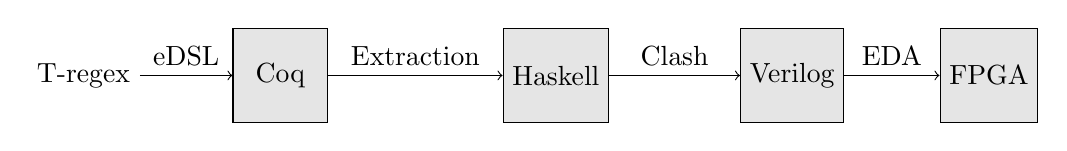
\begin{tikzpicture}[
  block/.style = {
    draw,
    shape=rectangle,
    minimum width=1.2cm,
    minimum height=1.2cm,
    fill=gray!20,
    align=center
  },
]
  \node (tregex) {T-regex};
  \node (coq)[
    right of=tregex,
    block,
    xshift=15mm
  ] {Coq};
  \node (haskell)[
    right of=coq,
    block,
    xshift=25mm
  ] {Haskell};
  \node (verilog)[
    right of=haskell,
    block,
    xshift=20mm,
    align=center
  ] {Verilog};
  \node (fpga)[
    right of=verilog,
    block,
    xshift=15mm,
    align=center
  ] {FPGA};

  \draw[->] (tregex) -- (coq) node[above,midway] {eDSL};
  \draw[->] (coq) -- (haskell) node[above,midway] {Extraction};
  \draw[->] (haskell) -- (verilog) node[above,midway] {Clash};
  \draw[->] (verilog) -- (fpga) node[above,midway] {EDA};
\end{tikzpicture}

% \end{document}
